\section{Models and Relationships}
The application defines several models to represent data:
\begin{itemize}
	\item \textbf{Function}: Represents a function that can be executed on the robot. Each function has a name and belongs to a category.
	\item \textbf{Command}: Represents a command that can be executed on the robot.one or more commands belong in one function which is executed by executing every single function one by one.
	\item \textbf{Category}: Represents a category to which functions belong. (MediaPipe, Visual Interaction, LiDAR )
	\item \textbf{FunctionCommand}: Represents the many-to-many relationship between functions and commands.
	\item \textbf{FunctionLibrary}: Represents the many-to-many relationship between functions and libraries.
	\item \textbf{FunctionCategory}: Represents the many-to-one relationship between functions and Category.
	
\end{itemize}

\begin{figure}[H]
	\centering
	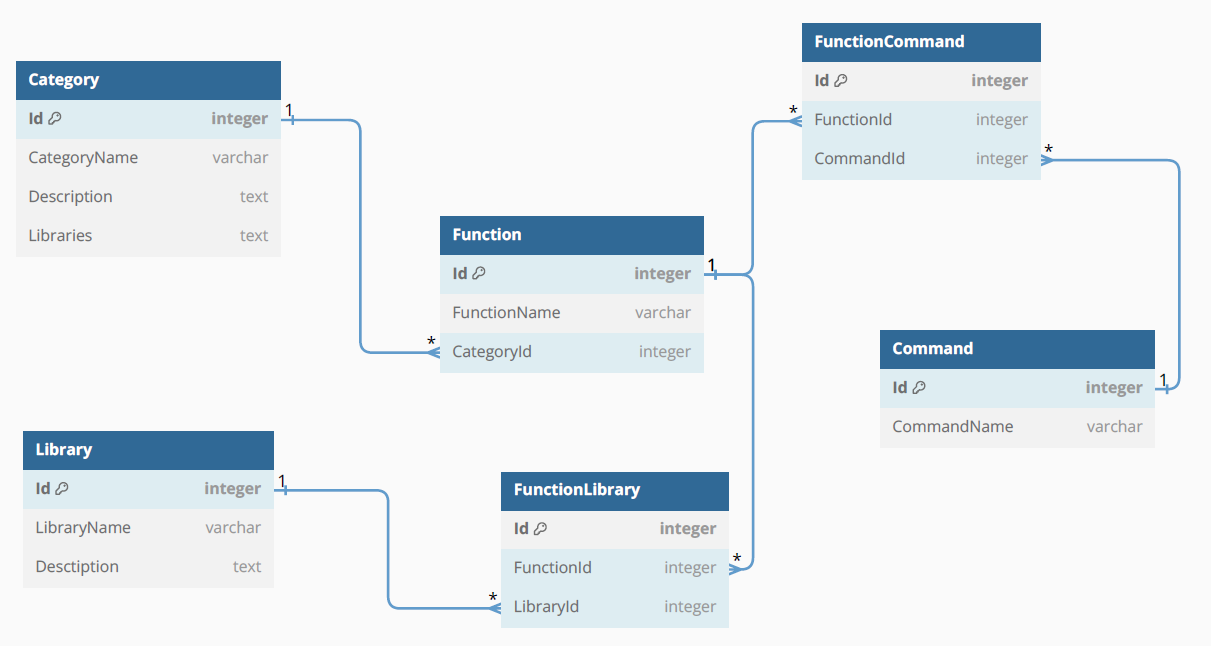
\includegraphics[width=1\textwidth]{Images/database.png}
	\caption{Database Relations}
	\label{}
\end{figure}
